\documentclass{beamer}       % print frames
%\documentclass[notes=only]{beamer}   % only notes
%\documentclass{beamer}              % only frames
\newcounter{savedenum}
\newcommand*{\saveenum}{\setcounter{savedenum}{\theenumi}}
\newcommand*{\resume}{\setcounter{enumi}{\thesavedenum}}
\usepackage{multienum}
\usepackage{minted}
\usepackage[notocbib]{apacite}
    \renewcommand{\APACrefatitle}[2]{#1}
    \renewcommand{\APACrefbtitle}[2]{#1}
    \renewcommand{\APACrefbtitle}[2]{\Bem{#1}}
    \renewcommand{\APACrefaetitle}[2]{[#2]}
    \renewcommand{\APACrefbetitle}[2]{[#2]} 
\usepackage{textpos}
\usepackage{setspace}
\usefonttheme{serif}
%\usepackage{graphicx}
\usetheme{Boadilla}
\usepackage{hyperref}
\usepackage[UKenglish]{babel}
\usepackage{multicol}
\setcounter{tocdepth}{1} 
\usecolortheme{orchid}
\title[ISFC Aachen 2015]{Discourse-semantics of risk in \emph{The New York Times}, 1963--2014: a corpus linguistic approach}
\author[Jens Zinn \and Daniel McDonald]{Zinn \& McDonald~\\~\\~\\This slideshow is available at: \url{http://git.io/vY0M4}~\\~\\}

\date{July 2015}

\begin{document}

\addtobeamertemplate{frametitle}{}{%
\begin{textblock*}{100mm}(.775\textwidth,-.5cm)

\includegraphics[scale=.235]{../images/unimelblong}
\end{textblock*}}

\frame{\titlepage}


\begin{frame}
    \frametitle{Presentation overview}
    
    \begin{itemize}
    \item Context of our investigation, research questions
    \item Sociological risk theory
    \item Linguistic approaches to risk
    \item Our methods and linguistic findings
    \item Sociological significance of the results
    \end{itemize}

    ~\\ This slideshow is available at: \url{http://git.io/vY0M4}

\end{frame}


\begin{frame}
    \frametitle{Context of our investigation}
    
    From previous sociological and linguistic research, we know that:

    \begin{itemize}
    \item Risk as concept is sociologically important (Beck, Giddens)
    \item Risk as lexical item is increasingly frequent in print journalism (Zinn 2011)
    \item \emph{Risk} as a lexical item in naturalistic text may behave contrary to expectations \cite{hamilton_meanings_2007}
    \end{itemize}
\end{frame}

\begin{frame}
    \frametitle{New methodologies}

    New kinds of data and tools make it possible to empirically analyse risk language in new ways:
    
    \begin{itemize}
    \item Digitisation of newspapers means we have large, well-structured datasets
    \begin{itemize}
        \item \emph{NYT Annotated Corpus}: 1.8 million articles, 1987--2007 \cite{sandhaus_new_2008}
    \end{itemize}
    \item Automatic annotation of text makes it possible to search for lexical and grammatical features in tandem
    \item Modern programming languages facilitate:
    \begin{itemize}
        \item Automation
        \item Reproducibility
        \item Transparency
    \end{itemize}
    \end{itemize}

\end{frame}


\begin{frame}
    \frametitle{Risk theory}
    
    \begin{itemize}
    \item The \emph{Risk Society} \cite{beck_risk_1992}
    \begin{itemize}
        \item Increased centrality of \emph{risk} in daily life in late modernity
        \item \emph{Mega risks}
        \item Individualisation of responsibility for managing risk
    \end{itemize}
    \item Technologisation: new data and tools for calculating risk and risk factors creates new functions of governments and institutions
    \item Risk vs. danger \cite{luhmann_ecological_1989}
    \end{itemize}
\end{frame}


\begin{frame}
    \frametitle{Research questions}

    We wanted to build on these earlier findings, and take advantage of new technologies:

    \begin{itemize}
        \item What are risk words doing in the NYT?
        \item How has the behaviour of risk words changed in the NYT between 1963 and 2014?
        \item Can we connect these findings to sociological theories of risk?
        \item What kinds of tools and methods can we use\slash develop to do this kind of research?
    \end{itemize}
\end{frame}

% daniel to take over here

\begin{frame}
    \frametitle{Frame semantic approach}

    Frame semantics: risk as a cognitive schema \cite{fillmore_toward_1992}

\begin{itemize}
    \item Conceptualises risk mostly as experiential Process\slash Event
    \begin{itemize}
        \item \emph{What kind of participants and circumstances occur when risk is the Process?}
    \end{itemize}
    \item Problem: risk often takes less prominent experiential roles
    \begin{itemize}
        \item Is the risk frame actually invoked when the word is used?
    \end{itemize}
    \end{itemize}

    ~\\
    \texttt{Mr. Tepfer noted that Mr. Douglas, who was in the neighborhood when the body was found and was interviewed by the police at the time, `preyed on \textbf{at-risk women}, on prostitutes, and he engaged in sex and strangled them to death.' }

\end{frame}

\begin{frame}
    \frametitle{Corpus linguistic approach}

    Corpus linguistics: risk as token \cite{hamilton_meanings_2007}

    \begin{itemize}
    \item Topics and text-types in which risk tokens appear
    \item Collocates of risk tokens \cite{hamilton_meanings_2007}
    \item Risk appears a lot in discussions of health
    \item Use of risk words is different to invented examples
    \end{itemize}

    Shortcomings:

    \begin{itemize}
        \item Smaller corpus size, heterogeneity of samples
        \item No parsing, lemmatisation
        \item No means of connecting lexicogrammar to meaning
    \end{itemize}

\end{frame}


\begin{frame}
    \frametitle{Our methods}
    
    \begin{itemize}
    \item Get all paragraphs containing \emph{risk} in all 1987--mid 2014 editions of the NYT:
    \begin{itemize}
    \item 153,828,656 words
    \item 149,504 articles
    \item 240,08 risk words
    \end{itemize}
    \item Annotate\slash parse the data for lemmata, constituency, dependency (not SFL!)
    \item Develop toolkit for manipulating the corpus and communicating results
    \begin{itemize}
        \item \url{https://www.github.com/interrogator/corpkit}
    \end{itemize}
    \item Interrogate the corpus
    \item Connect to sociological theory
    \end{itemize}
\end{frame}

%\begin{frame}
%    \frametitle{Constituency}
%    \centering
%    \includegraphics[width=0.75\textwidth]{../images/constituency}
%\end{frame}

\begin{frame}
    \frametitle{Dependency parsing}

    Q: Can we extract SF grammatical features from this? 

    ~\\

    \centering
    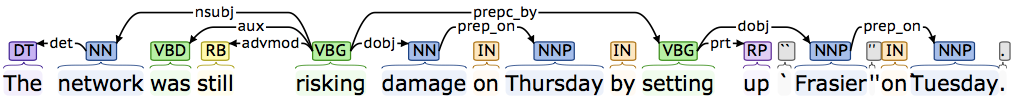
\includegraphics[width=0.99\textwidth]{../images/depparse}

    ~\\
    
    \raggedright
    A: Yes, quite often.
\end{frame}


\begin{frame}[fragile]
    \begin{minted}[fontsize=\footnotesize,linenos=true]{python}
# import module and define corpus path
from corpkit import *
nyt = 'data/nyt/years'

# count every pos
baseline = interrogator(nyt, 'pos', 'any', lemmatise = True)

# count pos for risk words
riskp = interrogator(nyt, 'pos', r'__ < /(?i)\brisk/', lemmatise = True)

# list open word classes
open_words = ['Noun', 'Verb', 'Adjective', 'Adverb']

# get relative frequencies of open word classes, skip 1963
maths_done = editor(riskp.results, '%', baseline.results, 
    sort_by = 'total', just_entries = open_words, 
    skip_subcorpora = [1963])

# plot
plotter('Percentage of open word classes that are risk words', 
    maths_done.results, legend_pos = 'lower left')
    \end{minted}
\end{frame}

\begin{frame}
    \frametitle{Output: nominalisation of risk}
    \centering
    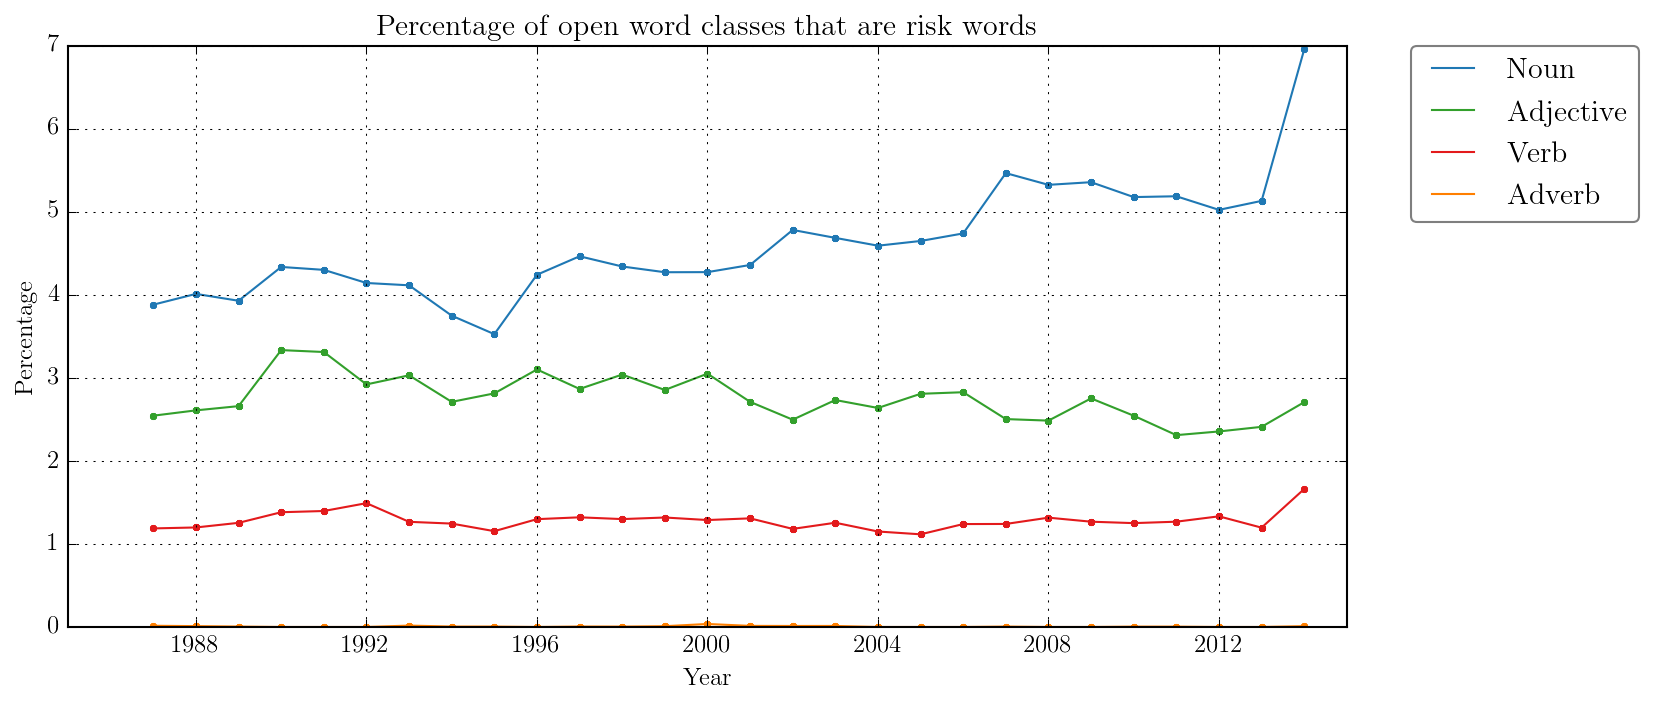
\includegraphics[width=0.99\textwidth]{../images/percentage-of-open-word-classes-that-are-risk-words}
\end{frame}

\begin{frame}
    \frametitle{Experiential roles of risk words}
    \centering
    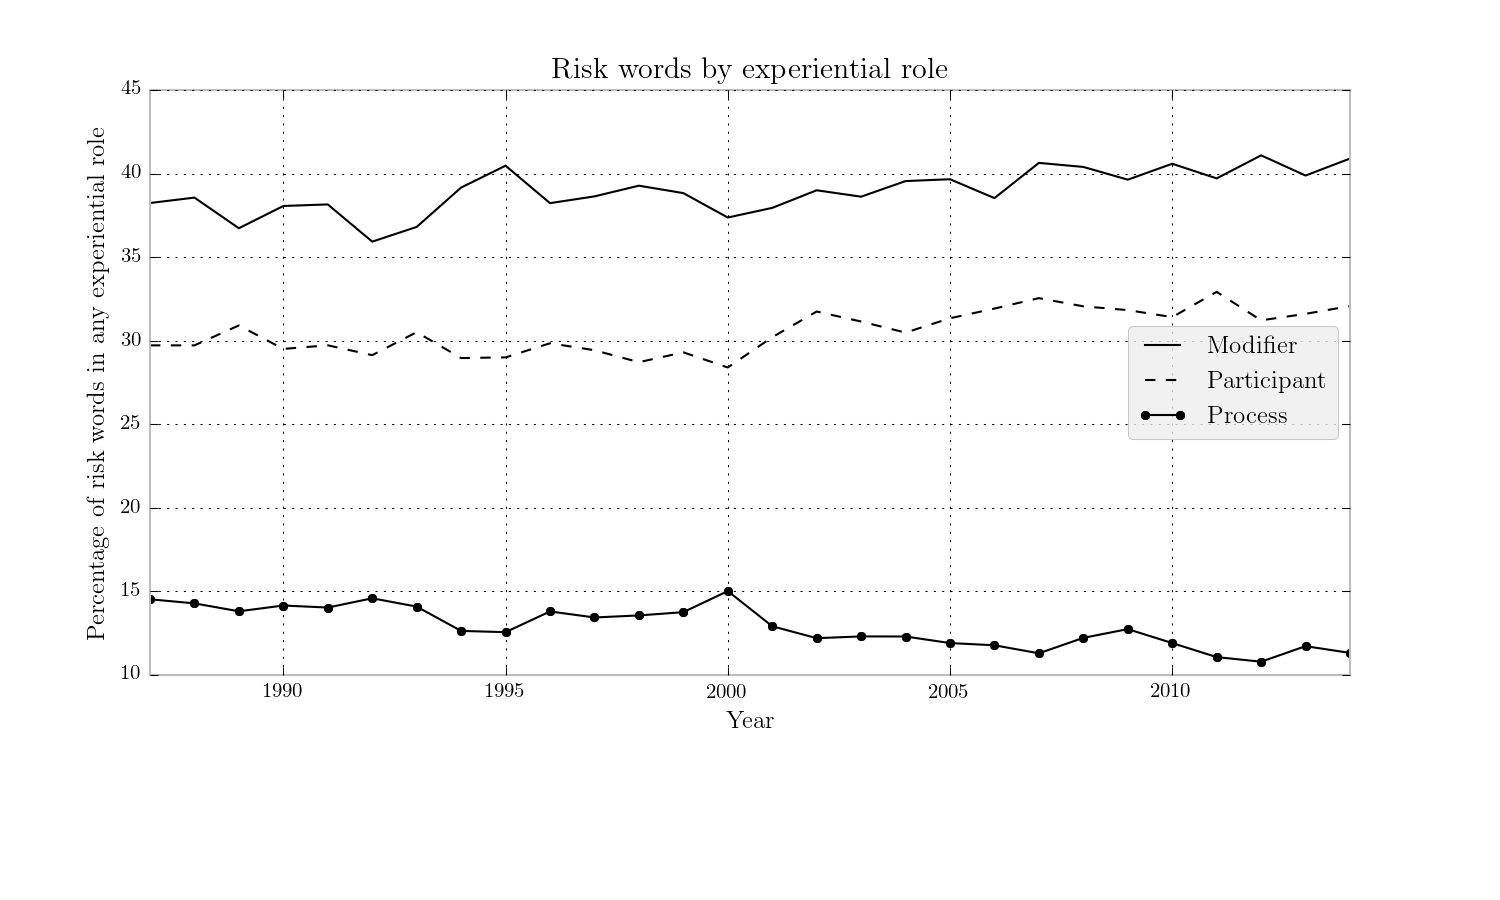
\includegraphics[width=0.99\textwidth]{../images/ppmfinal}
\end{frame}

\begin{frame}
    \frametitle{Risk as modifier}
    \centering
    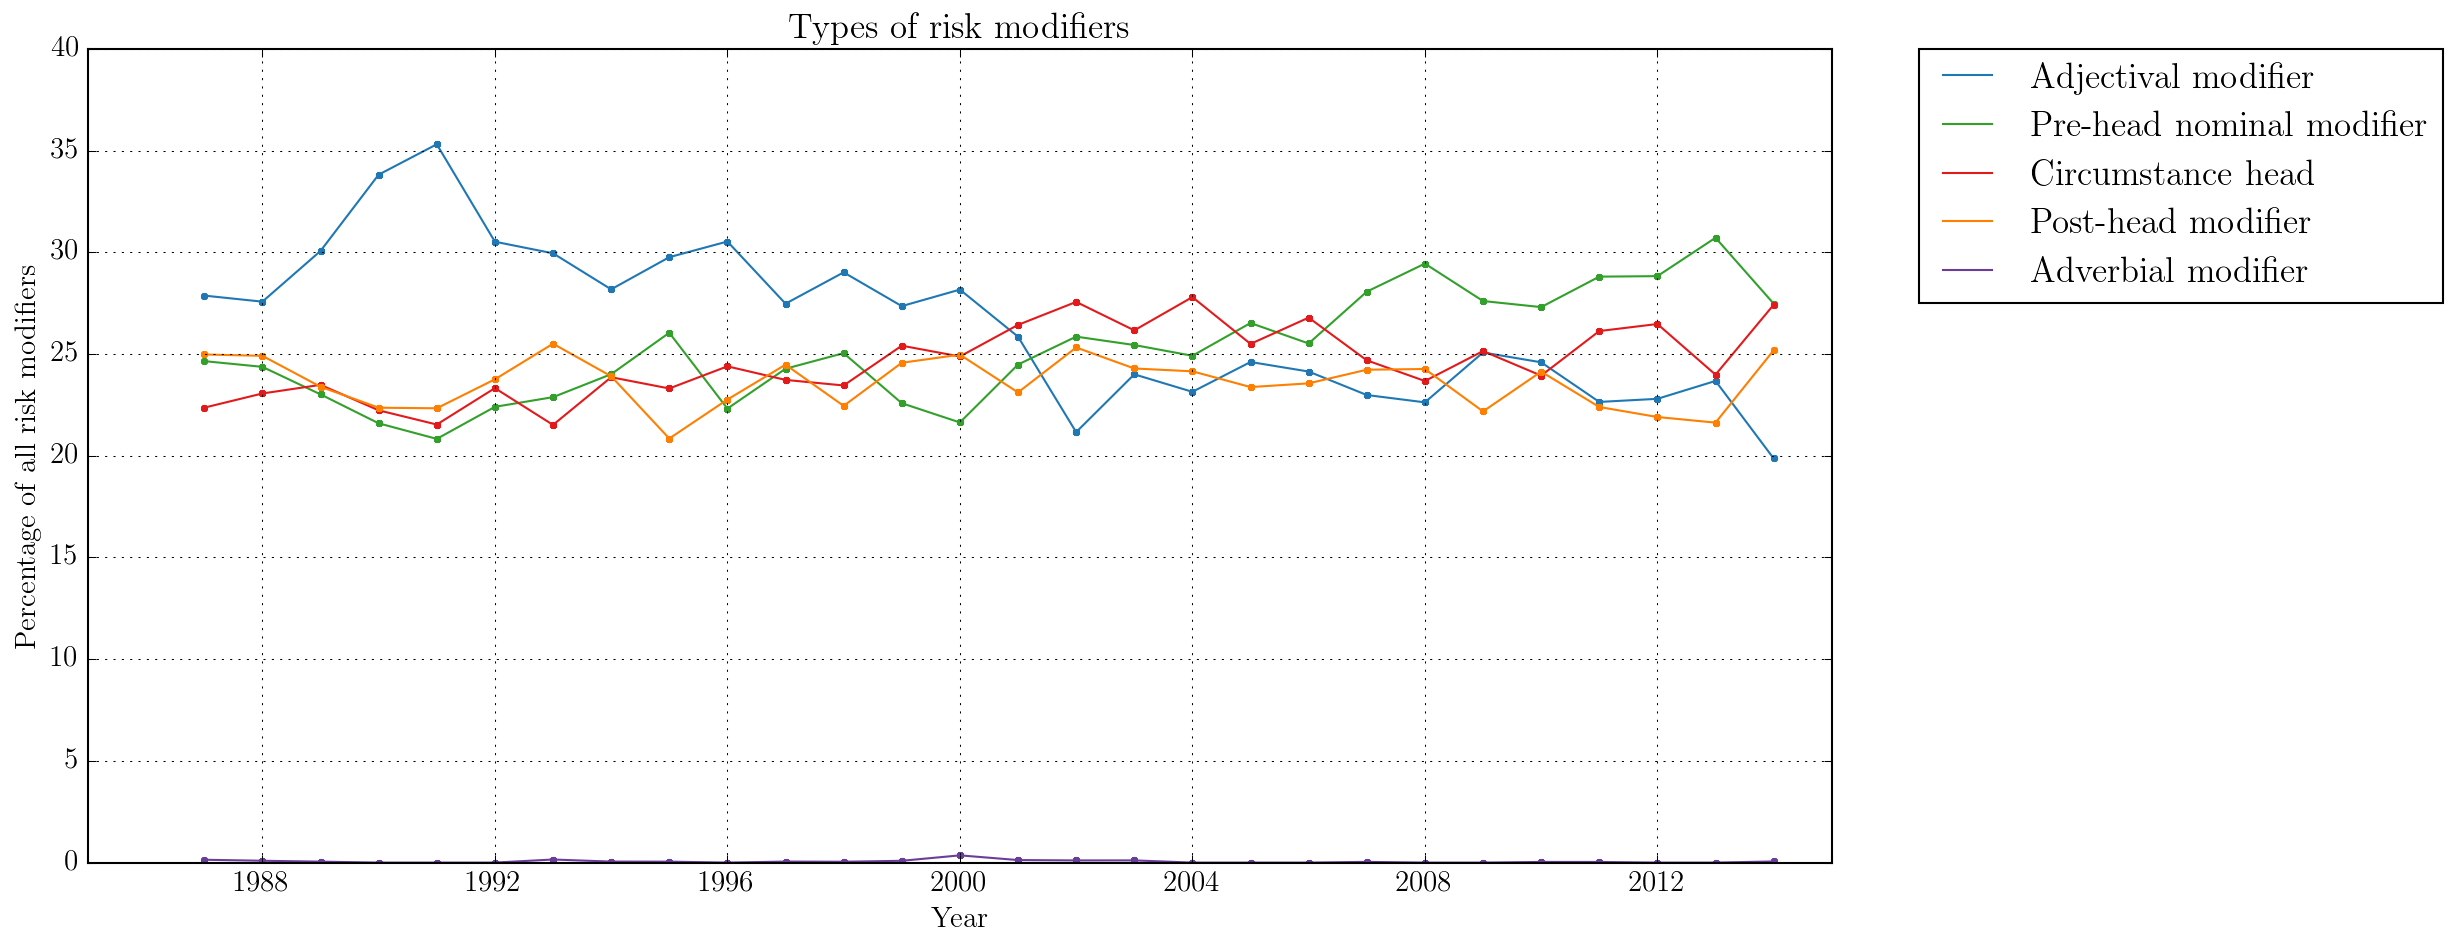
\includegraphics[width=0.99\textwidth]{../images/types-of-risk-modifiers}
\end{frame}

\begin{frame}
    \frametitle{Risk and power}
    \centering
    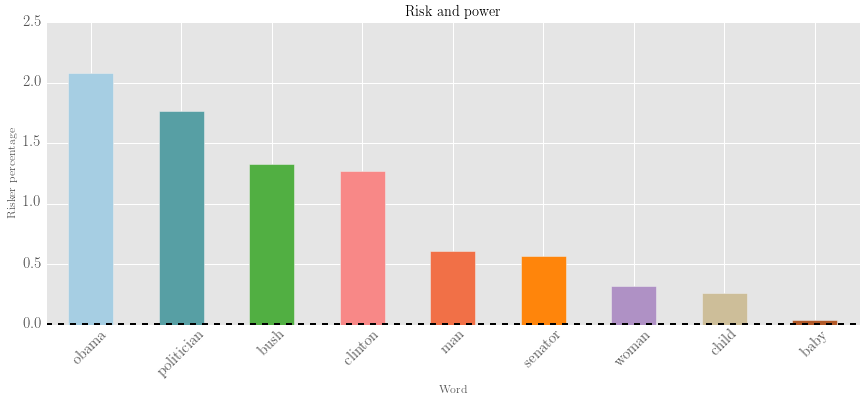
\includegraphics[width=0.99\textwidth]{../images/risk-and-power-2}
\end{frame}

\begin{frame}
    \frametitle{Mood role of risk words}
    \centering
    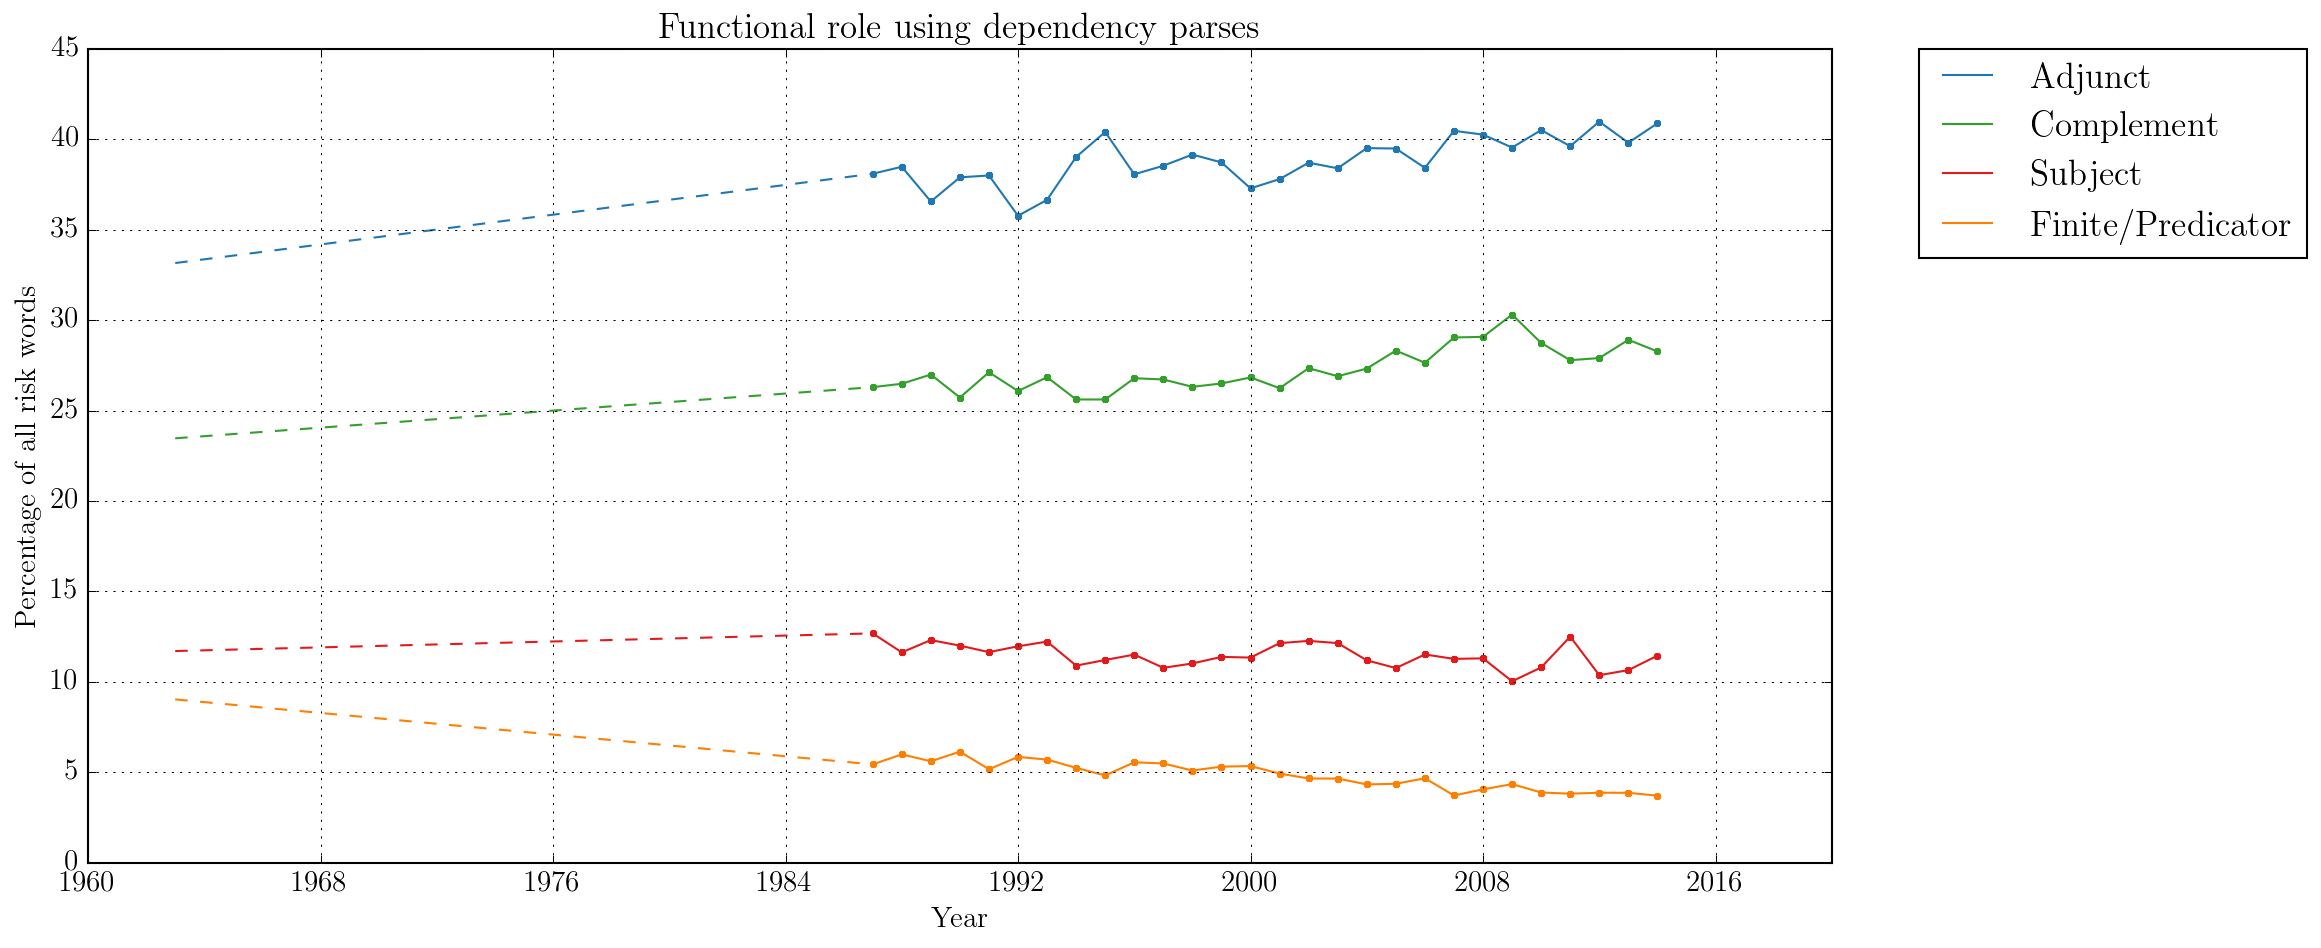
\includegraphics[width=0.99\textwidth]{../images/functional_role_using_dependency_parses}
\end{frame}

% \begin{frame}
%     \frametitle{Implicitness and arguability}
%     \centering
%     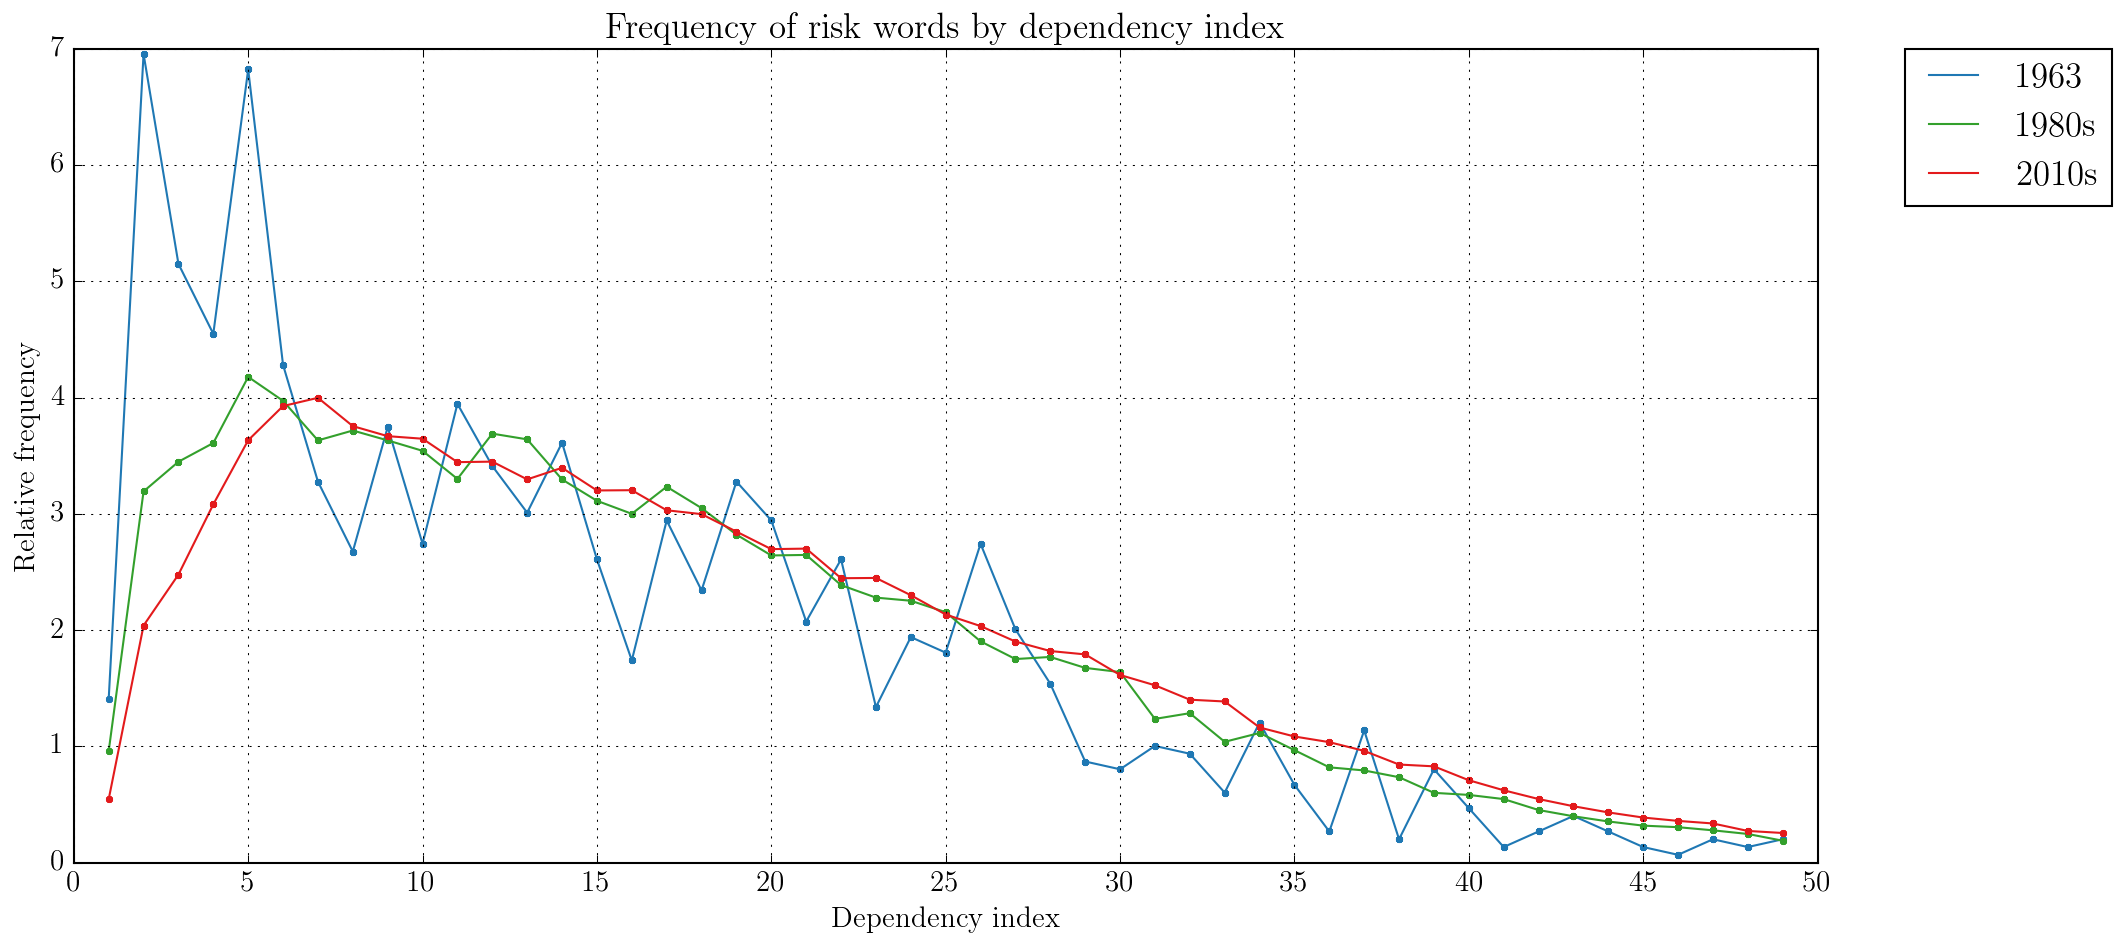
\includegraphics[width=0.99\textwidth]{../images/frequency-of-risk-words-by-dependency-index.png}
% \end{frame}

\begin{frame}
    \frametitle{Summary of key findings}
    
    \begin{itemize}
    \item Nominalisation and participantification
    \item Risk words becoming more implicit
    \item More everyday exposure to risk, but less risking
    \item Complicated constellations of participants and circumstances in risk processes
    \end{itemize}
\end{frame}

\begin{frame}
    \frametitle{Discussion of methodology}
    
    \begin{itemize}
    \item SFL proves a useful means of dividing up and investigating the behaviour of a given word
    \item SFL parsing is difficult, as is converting concepts from (esp. formal) grammars
    \item That said, though theoretical orientations are different, much of the grammar (esp. at group\slash phrase levels) are similar
    \end{itemize}
\end{frame}


\begin{frame}
    \frametitle{Sociological discussion}

    There are points of convergence, as well as disparities between, our linguistic findings and influential sociological theories:
    
    \begin{itemize}
    \item 
    \item 
    \item 
    \item 
    \end{itemize}

\end{frame}

\begin{frame}
    \frametitle{Research agenda}
    \begin{itemize}
        \item Further exploration of risk as per SFG: process types, mood features, thematic metafunction
        \item New datasets and comparative analyses
        \item Expanding our focus to related terms: \emph{danger}, \emph{(in)security}, etc.
    \end{itemize}
\end{frame}


\begin{frame}
    \frametitle{We're open source}

    Data and tools are available for reuse:
    \begin{itemize}
    \item \url{https://www.github.com/interrogator/risk}
    \end{itemize}
    Findings are presented dynamically in an IPython Notebook: 
    \begin{itemize}
    \item \url{http://git.io/vIM2W}
    \end{itemize}
    This slideshow:
    \begin{itemize}
    \item \url{http://git.io/vY0M4}
    \end{itemize}
\end{frame}








    \begin{frame}[t,allowframebreaks]
    \frametitle{References}
    \bibliographystyle{apacite}
    \bibliography{references/references}
    \end{frame}
    
    \end{document}